
\section{Введение}
В последние годы влияние Интернета на жизнь человека становится все сильнее. Это обусловлено тем, что Интернет предоставляет гораздо больше удобства и возможностей для доступа к информации. Не оказалась в стороне от Интернета и такая важная часть работы и досуга, как чтение книг.

Двадцать лет назад для того, чтобы найти книгу человек шел в библиотеку или в книжный магазин. Если он искал определённую книгу --- достаточно было назвать фамилию автора и название книги, а порой даже одного названия было достаточно. Если же выбор книги ещё не был сделан, всегда можно было получить помощь от сотрудника магазина или библиотеки. Сегодня ситуация с библиотеками и книжными магазинами изменилась несильно, но наравне с бумажными книгами появилась возможность читать книги в электронном виде. 

Большое количество книг оцифровано и хранится в сети Интернет, многие из них находятся в свободном доступе. С одной стороны, это должно упрощать процесс получения книг, \tk теперь они стали доступны из любого места, где есть возможность выхода в Интернет. С другой стороны, перед пользователем встает новые проблемы. Во-первых, теперь ему необходимо самому искать книгу в сети, где количество информации растет с каждым днем. Во-вторых, после того, как он нашел нужную книгу --- ее нужно скачать, а затем найти программу, которая позволяет читать файл в найденном формате. 

На настоящий момент в Интернете существует множество электронных библиотек, поиск по которым весьма затруднен из-за того, что не существует системы, которая могла бы объединить всю информацию с этих библиотек. Следовательно, пользователям приходится либо искать в каждой из электронных библиотек в отдельности, либо пользоваться существующими поисковыми системами. Есть еще одна проблема, связанная с наличием большого количества электронных библиотек. Она состоит в том, что единый формат для предоставления информации о книгах появился только недавно, поэтому каждая библиотека предоставляет свой формат.

У существующих поисковых систем, в свою очередь,  есть одна очень важная особенность --- они обладают ограниченными возможностями в проведении специализированного поиска в сети. Поэтому в результате поиска пользователь получает всю информацию, которая соответствует поисковому запросу и дальше уже начинается работа самого пользователя над тем, чтобы эту информацию профильтровать и извлечь оттуда именно то, что ему нужно. 

Таким образом, выявляются две важные проблемы, затрудняющие поиск книг. Первая проблема --- различные библиотеки имеют разные интерфейсы, вторая --- существует множество форматов, в которых может быть представлена электронная книга. 

В данной работе была разработана система, упрощающая задачу поиска, чтения и управления книгами. 


\section{Обзор существующих решений}

Все эти проблемы не новы и попытки решить эти проблемы уже предпринимались.

Например, широко известная поисковая система Google предоставляет свой сервис для поиска электронных книг --- Google books (\url{http://books.google.com}). Этот сервис выполняет полнотекстовый поиск по книгам, которые Google сканирует и сохраняет в своей базе данных. В качестве результатов поиска выдается большое количество информации о самой книге, о различных изданиях этой книги и ссылки на ресурсы, где пользователь может приобрести книгу. Благодаря полнотекстовому поиску  по содержанию, есть возможность найти книгу, имея сильно ограниченное количество информации о ней. Этот сервис не решает ни проблему унифицированного доступа к информации о книгах, ни проблему различных форматов книг.

Сайт \url{http://ebdb.ru} (electronics books data base)  --- это поисковая система, которая обходит интернет и сохраняет у себя ссылки на те страницы сторонних ресурсов, которые содержат ссылки на книги. В результате поиска выдается список ссылок на страницы, содержащие книги. Для того, чтобы получить книгу пользователь должен перейти по ссылке, и, возможно, зарегистрироваться на ресурсе. Это решает проблему поиска книг, находящихся в свободном доступе, но остаются другие задачи, которые пользователь вынужден выполнять самостоятельно (скачивание книг и поиск подходящей программы для просмотра). Эта поисковая система тоже не решает проблемы унифицированного доступа и проблему различных форматов книг.

Есть большие системы, решающие проблему унифицированного доступа и различных форматов книг, а именно, Amazon Kindle, Sony Reader и подобные. 
Это программно-аппаратные платформы для чтения электронных книг. Они предоставляют устройство, которое имеет доступ к определенному хранилищу. Пользователь может подключить свое устройство к Интернету, найти нужную книгу в этом хранилище и купить ее. Дальше устройство само скачает книгу и откроет ее.
Из минусов у таких систем то, что эти системы платные и зависимые от устройства. Количество доступных книг --- ограничено теми книгами, которые хранят/продают хранилища, к которым они подключаются. Но это не единственные минусы таких систем. Так, к примеру, у Amazon Kindle за каждый загруженный текст (вне зависимости от источника загрузки) требуется заплатить компании Amazon от 10 центов. Еще Amazon контролирует информацию, содержащуюся на устройствах, находящихся у пользователей и по своему усмотрению удаляет её (в том числе книги, приобретённые непосредственно у Amazon).

Существует открытая технология, решающая проблему унифицированного доступа  --- OPDS (Open Publication Distribution System).
OPDS --- это новый активно развивающийся стандарт, который построен на базе расширяемого языка разметки Atom. Этот стандарт был специально разработан для предоставления информации об электронных документах. В нем учтены особенности такого рода информации (наличие аннотации, автора, изображения обложки и пр.).
Основная идея существования такого стандарта в том, что если многие сайты будут распостранять свою информацию о книгах в таком формате, то клиентские программы могут работать с ними единообразно (см. \picref{fig:scheme}). Несмотря на то, что стандарт появился недавно, уже существуют сайты и клиетские программы, использующие этот протокол. 

\begin{figure}
\centering
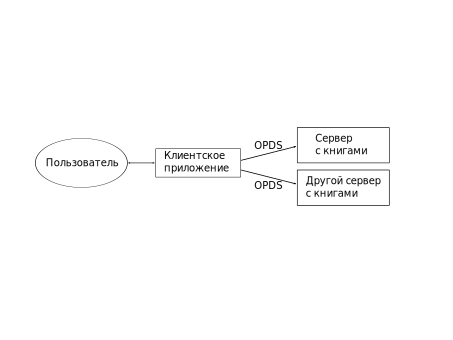
\includegraphics[width=.5\textwidth]{scheme}
\caption{Схема взаимодействия с использованием формата OPDS}\label{fig:scheme}
\end{figure}

Одим из самых крупных сайтов, предоставляющих информацию по протоколу OPDS, является BookServer (\url{http://bookserver.archive.org}).
Этот некоммерческий проект является частью проекта Internet Archive (\url{http://archive.org}) и является универсальной и открытой системой распостранения электронных книг. BookServer это архитектура, объединяющая различные форматы книг, конвертируя их, при необходимости, в нужный формат. Система обеспечивает каталогизацию книг, имеющихся в магазинах, библиотеках или в открытом доступе. Электронный текст можно прочитать на любом конечном устройстве, будь то нетбук, смартфон или специализированное устройство для чтения, наподобие Kindle. Хотя сайтом уже можно пользоваться, он еще находится на стадии разработки, с чем, вероятно, связано отсутствие расширенного поиска по книгам, фильтрации по языкам/жанрам. Так же, минусом этого проекта для русскоговорящих пользователей является невозможность поиска с использованием русских символов.

%TODO BEGIN
\section{Описание системы в целом}
Проект состоит из серверной и клиентской частей.

Серверная часть собирает в сети Интернет информацию об электронных книгах и представляет собранную информацию для обычных пользователей в виде web-интерфейса и для клиентских программ --- в формате OPDS.

Клиентская часть представляет собой программу для удобной работы с сервером, предоставляющим по запросам информацию в формате OPDS. Клиент должен работать как с "родным" сервером, так и с другими серверами, поддерживающими OPDS, например feedbooks.com.
Пользователь устанавливает у себя на машине одну из клиентских программ. При поиске книги программа обращается к одному из серверов, поддерживающих протокол OPDS. Сервер обрабатывает запрос, и возвращает данные в в нужном формате. 

Клиентских программ написано 2:
\begin{enumerate}
	\item На С++ (с использованием библиотеки Qt)
	\item На Java
\end{enumerate}

Серверная часть проекта состоит из 3 подпроектов:
\begin{enumerate}
	\item сборщик информации в сети (crawler) (java)
	\item анализатор найденной информации, разбирающий информацию о книгах (java) 
	\item собственно web-сервер, включающий базу данных, поиск по ней, представление информации в web и opds форматах (python, django)
\end{enumerate}

Web-серевер, в свою очередь, состоит из двух частей. Первая, внутренняя часть, обеспечивает поиск информации по базе и взаимодействие с анализатором.
Вторая, внешняя часть, предроставляет информацию и занимается сбором дополнительной. Информация предоставляется двумя способами: в виде web-интерфейса для пользователя и по протоколу OPDS для клиентских программ.


%Клиентская программа на Java более переносима, но для нее необходимо на девайсе иметь java-машину. В свою очердь программа на Qt не требует установки никаких дополнительных библиотек, работает быстрее, но переносимость ниже, чем у java.
		
\section{Описание внустренней структуры системы}
Crawler обходит Интернет в поисках электронных книг в различных форматах. Если он нашёл нечто, похожее на книгу, он передаёт ссылку на этот объект и ссылку на страницу, на которой он нашёл ссылку на книгу.
После этого анализатор пытается распознать: дейсвительно ли это книга, какое у неё название, авторы. На этом этапе, аналайзер ипользует как свой внутренний механизм, так и информацию о книгах, авторах хранящуюся на сервере. Для этого он использует специальный интерфейс, предлагаемый сервером.
Если анализатор распознал в полученом объекте книгу, то далее он пытается понять, существует ли на сервере автор данной книги, существует ли такое произведение. Эта задача нетривиальна, так как в различных файлах одной и той же книги написание названия/имёна авторов могут различаться.
После упешного распознавания, аналайзер добаляет информацию о файле и ссылку на него в базу на сервер. Используя для этого специальный интерфейс модифкации данных, предлагаемый сервером.
Теперь информация о книге хранится на сервере и доступна через web-интерфейс или в OPDS формате.
% Может стоит вставить пару картинок


% TODO STOP
